\documentclass{beamer}
\usepackage[spanish]{babel}
\usepackage[latin1]{inputenc}
\usepackage{multicol} % indice en 2 columnas
\usepackage{centernot}
\usepackage{amsmath}% http://ctan.org/pkg/amsmath

\usepackage{color}


\usepackage{graphicx}
\graphicspath{ {im/} }


\newcommand{\notimplies}{%
  \mathrel{{\ooalign{\hidewidth$\not\phantom{=}$\hidewidth\cr$\implies$}}}}


\usetheme{Warsaw}
%\usecolortheme{crane}
\useoutertheme{shadow}
\useinnertheme{rectangles}

\setbeamertemplate{navigation symbols}{} % quitar simbolitos

\title[Tema 8 - Introducci\'on a la Teor\'ia de Grafos]{Teor\'ia de grafos}
\subtitle{Estudios de Ingenier\'ia}
\author[https://frogames.es]{
Juan Gabriel Gomila%$^{1}$  \and E. Eva$^{2}$ \and S. Serpiente$^{3}$
}
\institute[Frogames]{
 % $^{1-2}$
 Frogames
   \and
  \texttt{https://frogames.es}
}
\date{\today}


\AtBeginSection{
\begin{frame}
  \begin{multicols}{2}
  \tableofcontents[currentsection]   
\end{multicols}
\end{frame}
}

\AtBeginSubsection{
\begin{frame}
  \begin{multicols}{2}
  \tableofcontents[currentsection,currentsubsection]
\end{multicols}
\end{frame}
}



%empieza aqui


\begin{document} 

\frame{\titlepage}

\begin{frame}
  \frametitle{\'Indice}
  \tableofcontents
\end{frame}

\section{Teor\'ia de grafos}
\subsection{Un poco de historia}


\begin{frame}
\frametitle{Origen de los grafos}
La teor\'ia de grafos es una rama de la matem\'atica que surge y se desarrolla para dar soluciones a problemas muy concretos. 

El problema que la mayor\'ia de autores se\~nalan como el origen de la teor\'ia de grafos es el \textbf{problema de los puentes de K\"onigsberg}


\begin{figure}[h]
 \label{fig:volumen}
\centering
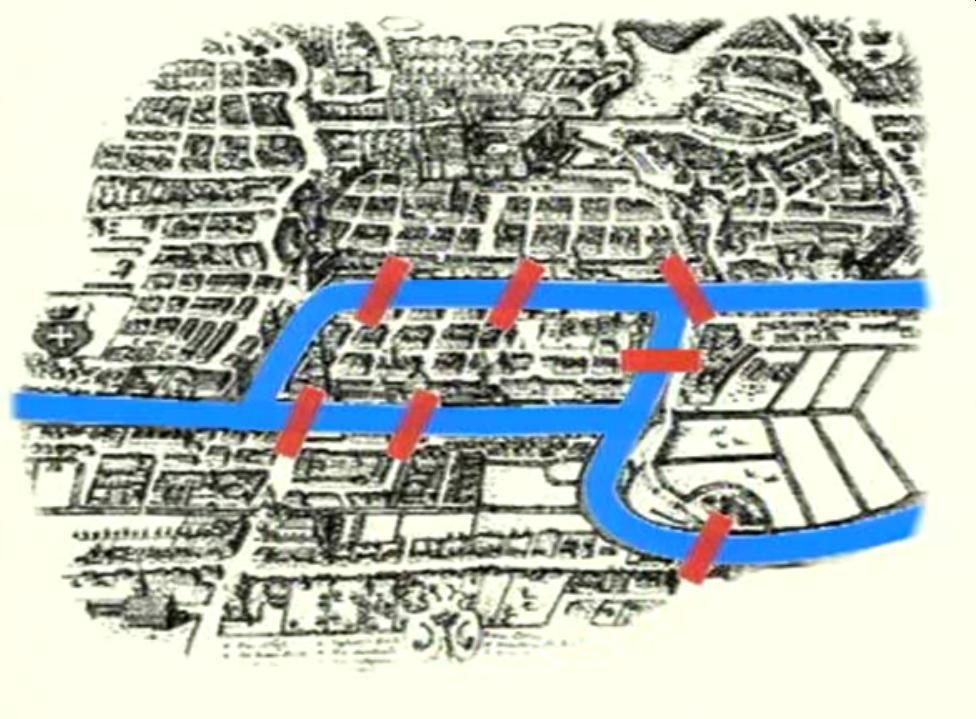
\includegraphics[height=5cm]{konisgberg}
\end{figure}
 
\end{frame}

\begin{frame}
\frametitle{Origen de los grafos}
Durante el siglo XVIII, la ciudad de K\"onigsberg (Prusia Oriental) estaba dividida en cuatro zonas por el rio Prevel. Hab\'ia siete puentes que comunicaban estas regiones como demuestra el dibujo:
\begin{figure}[h]
 \label{fig:volumen}
\centering
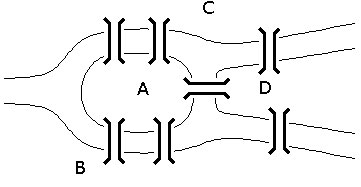
\includegraphics[height=5cm]{kon2}
\end{figure}
\end{frame}


\begin{frame}
\frametitle{Origen de los grafos}
Los habitantes de la ciudad no ten\'ian ni BioFestes ni Univerlands, en lugar de tener vuestras mismas necesidades, necesitaban encontrar una manera de pasear por la ciudad que les permitiera ir a una determinada regi\'on, cruzar cada puente una \'unica vez y volver al lugar de partida. 
\begin{figure}[h]
 \label{fig:volumen}
\centering

\includegraphics[height=4.8cm]{univerland}
\end{figure}
\end{frame}


\begin{frame}
\frametitle{Origen de los grafos}
Para resolver este problema, Euler represent\'o las cuatro zonas de la ciudad por cuatro puntos y los puentes por aristas que uniesen los puntos, tal y como se ve en la figura:
\begin{figure}[h]
 \label{fig:volumen}
\centering
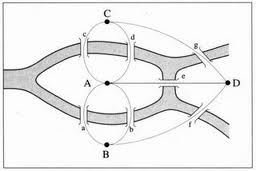
\includegraphics[height=4.8cm]{kon3}
\end{figure}
\end{frame}


\begin{frame}
\frametitle{Origen de los grafos}
Actualmente, la teor\'ia de grafos se aplica dentro y fuera de las matem\'aticas y sigue siendo un rama de investigaci\'on muy activa. Sus aplicaciones son muy importantes en la ingenier\'ia y resultan de gran utilidad para la representaci\'on de datos, dise\~no de redes de telecomunicaci\'on...
\end{frame}


\section{El concepto de grafo}


\begin{frame}
\frametitle{?`Qu\'e es un grafo?}
Los grafos se pueden considerar formalmente como diagramas (representaciones geom\'etricas) o bien algebraicamente como un par de conjuntos (representaci\'on algebraica). V\'eanse ambos tipos de definiciones:
\end{frame}

\subsection{Definici\'on geom\'etrica del grafo}
\begin{frame}
\frametitle{Definici\'on geom\'etrica del grafo}
\begin{block}{Definici\'on}
Geom\'etricamente, un grafo $G$ es un conjunto de puntos del espacio, algunos de los cuales est\'an unidos entre ellos mediante l\'ineas. 
\end{block}
Este grafo puede simbolizar por ejemplo un mapa de carreteras donde los puntos representan ciudades y las l\'ineas, las carreteras que las unen. En este caso, el grafo puede informar de las posibles comunicaciones que existen entre las ciudades, pero este grafo $G$ tambi\'en podr\'ia esquematizar un circuito el\'ectrico. 

\begin{figure}[h]
 \label{fig:volumen}
\centering
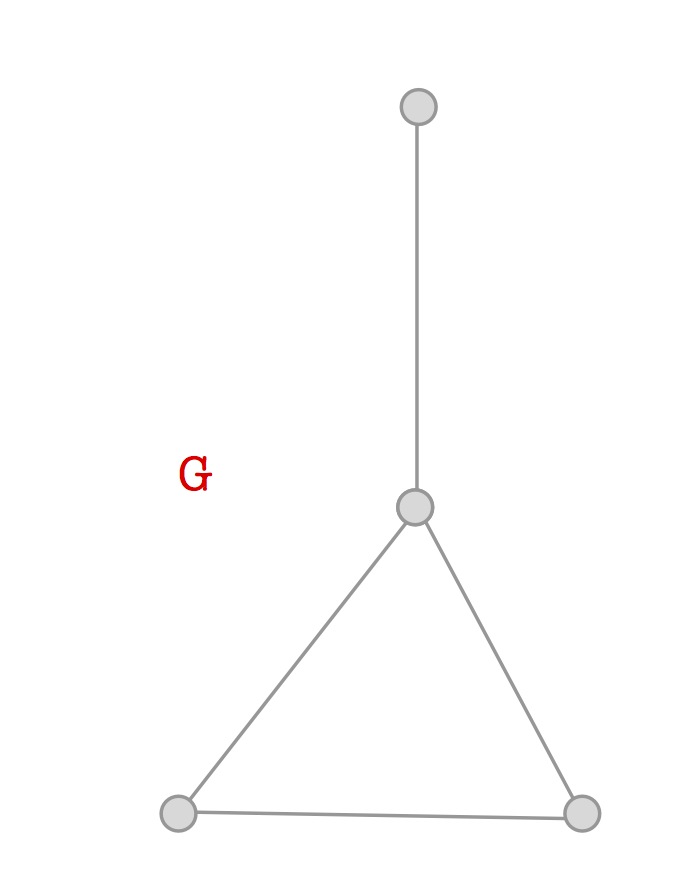
\includegraphics[height=3cm]{g1}
\end{figure}\end{frame}





\begin{frame}
\frametitle{Definici\'on geom\'etrica del grafo}

Se ha de hacer constar que un grafo solo contiene informaci\'on sobre la conectividad entre puntos y no da informaci\'on geom\'etrica en sentido eucl\'ideo (distancias, \'angulos...). As\'i los siguientes diagramas representan el mismo grafo.

\begin{figure}[h]
 \label{fig:volumen}
\centering
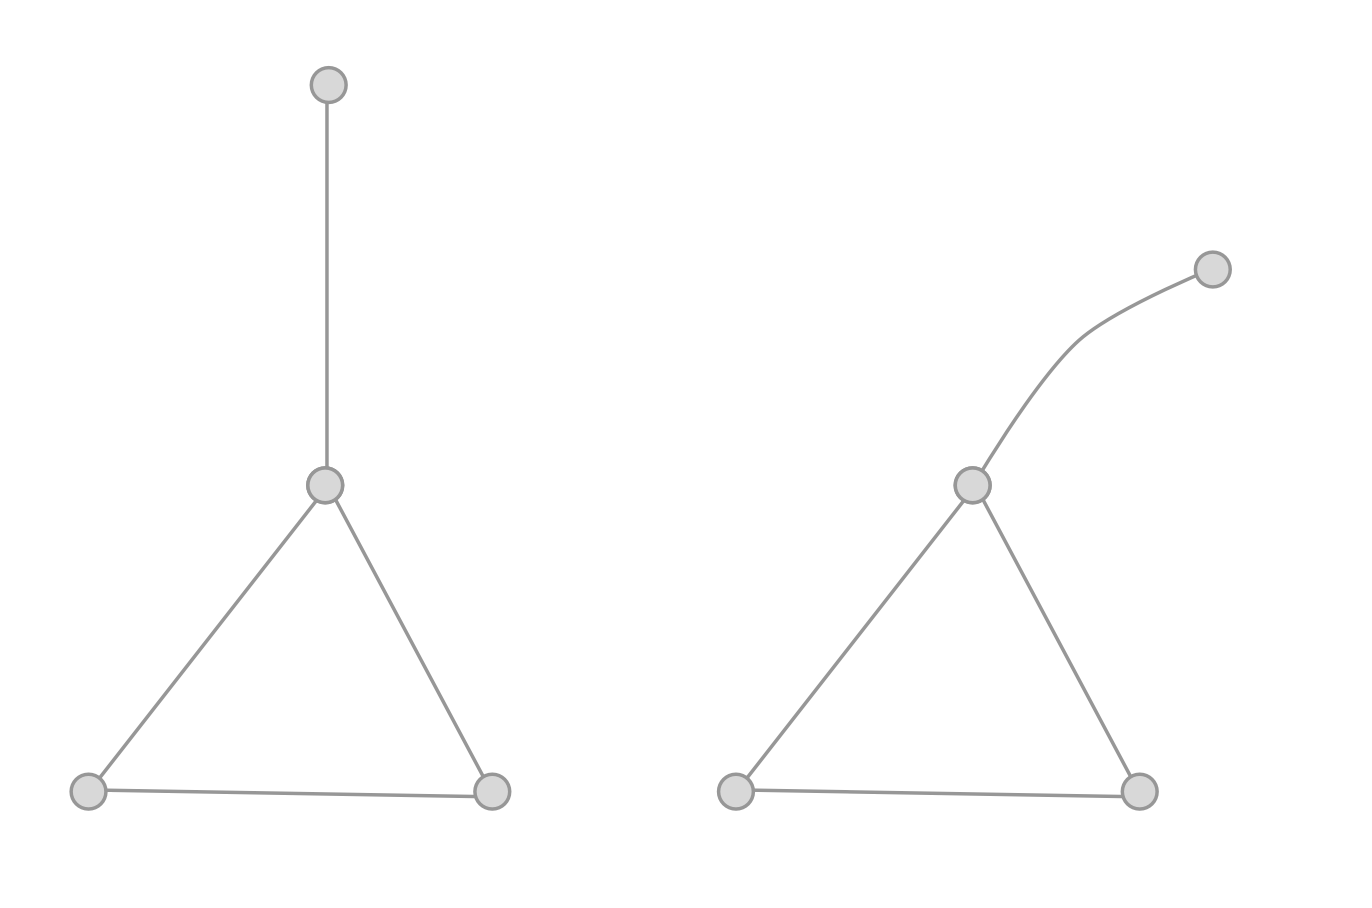
\includegraphics[height=4cm]{g2}
\end{figure}
\end{frame}



\subsection{Definici\'on algebraica del grafo}
\begin{frame}
\frametitle{Definici\'on algebraica del grafo}

\begin{block}{Definici\'on}
Un grafo $G$ se define como un par ordenado de conjuntos $G=(V,E) = (V(G), E(G))$ donde:
\begin{itemize}
\item $V$ es un conjunto no vac\'io de puntos $V=\{v_1,v_2,\cdots,v_n\}$ denominados \textbf{v\'ertices}, y
\item $E$ es un conjunto de pares no ordenados de elementos de $V$, denominados \textbf{aristas}
\end{itemize}
\end{block}
Si dos v\'ertices $u,v$ est\'an unidos por la misma arista, entonces d\'icese que son \textbf{adyacentes} y se representan por su arista por $\{u,v\}$

En este caso tambi\'en se dir\'a que $u$ y $v$ son \textbf{incidentes} a la arista $\{u,v\}$

\end{frame}




\begin{frame}
\frametitle{Definici\'on algebraica de grafo}
Para representar algebraicamente un grafo es necesario poder distinguir los v\'ertices y las aristas. As\'i:

\begin{figure}[h]
 \label{fig:volumen}
\centering
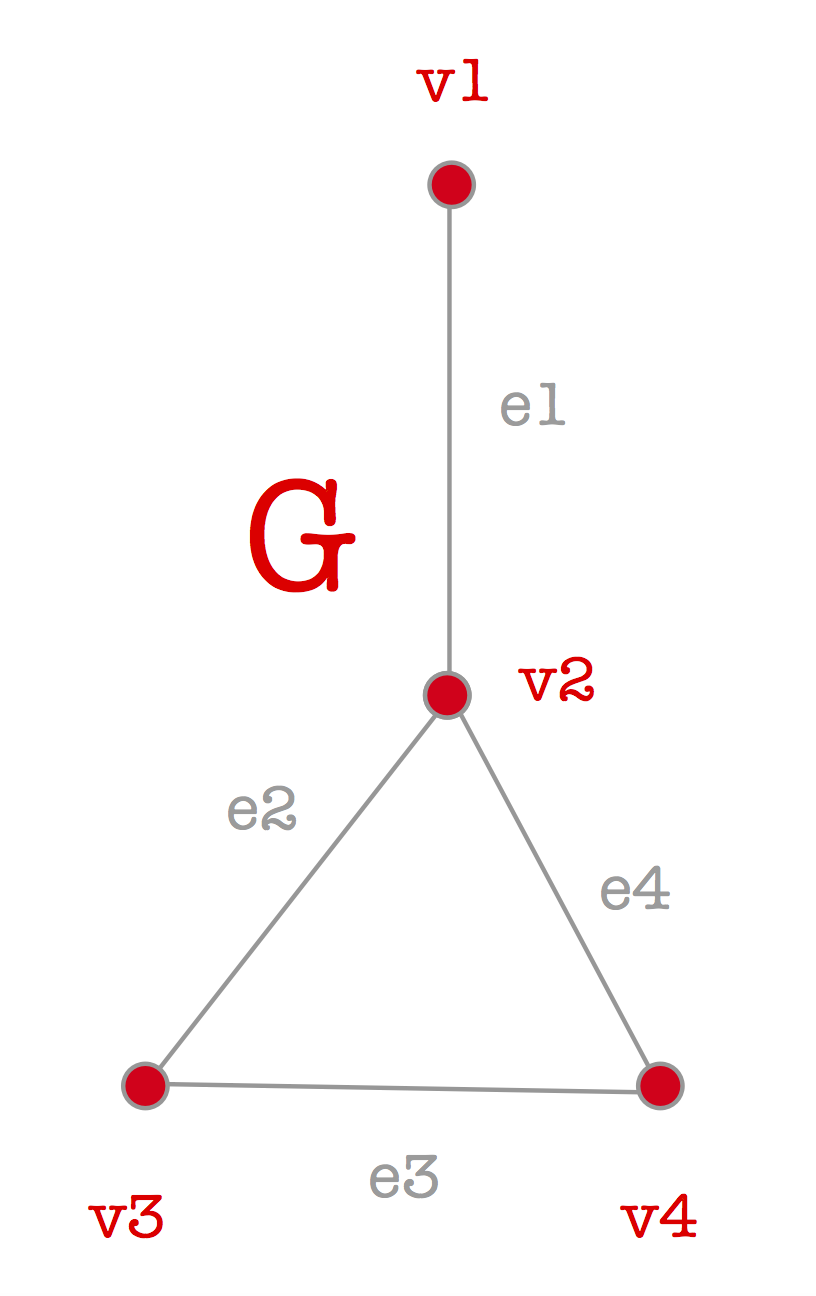
\includegraphics[height=4cm]{g3}
\end{figure}
\[G=(V(G),E(G))\]
\[V = V(G) = \{v_1,v_2,v_3,v_4\};\ \ E = E(G) = \{e_1,e_2,e_3,e_4\}\]
Donde $e_1 = \{v_1,v_2\}, e_2 = \{v_2,v_3\}, e_3 = \{v_3,v_4\}, e_4 = \{v_2,v_4\}$
\end{frame}









\begin{frame}
\frametitle{Definici\'on algebraica de grafo}

\begin{block}{Definiciones}
\begin{itemize}
\item El n\'umero de v\'ertices del grafo $G$, $|V(G)|$ se denomina el \textbf{orden del grafo}. 
\item El n\'umero de aristas del grafo $G$, $|E(G)|$ se denomina el \textbf{tama\~no del grafo}.
\end{itemize}
\end{block}

\begin{block}{Grafo trivial}
 Un grafo $G$ es finito si $|V(G)|$ y $|E(G)|$ son finitos. Si un grafo finito tiene un v\'ertice y no tiene ninguna arista, nos referiremos a \'el como grafo trivial (corresponde a un solo punto)
\end{block}
\end{frame}





\begin{frame}
\frametitle{Definici\'on algebraica de grafo}

\begin{block}{Ejemplo}
El siguiente diagrama no corresponde a un grafo ya que contiene:
\begin{figure}[h]
 \label{fig:volumen}
\centering
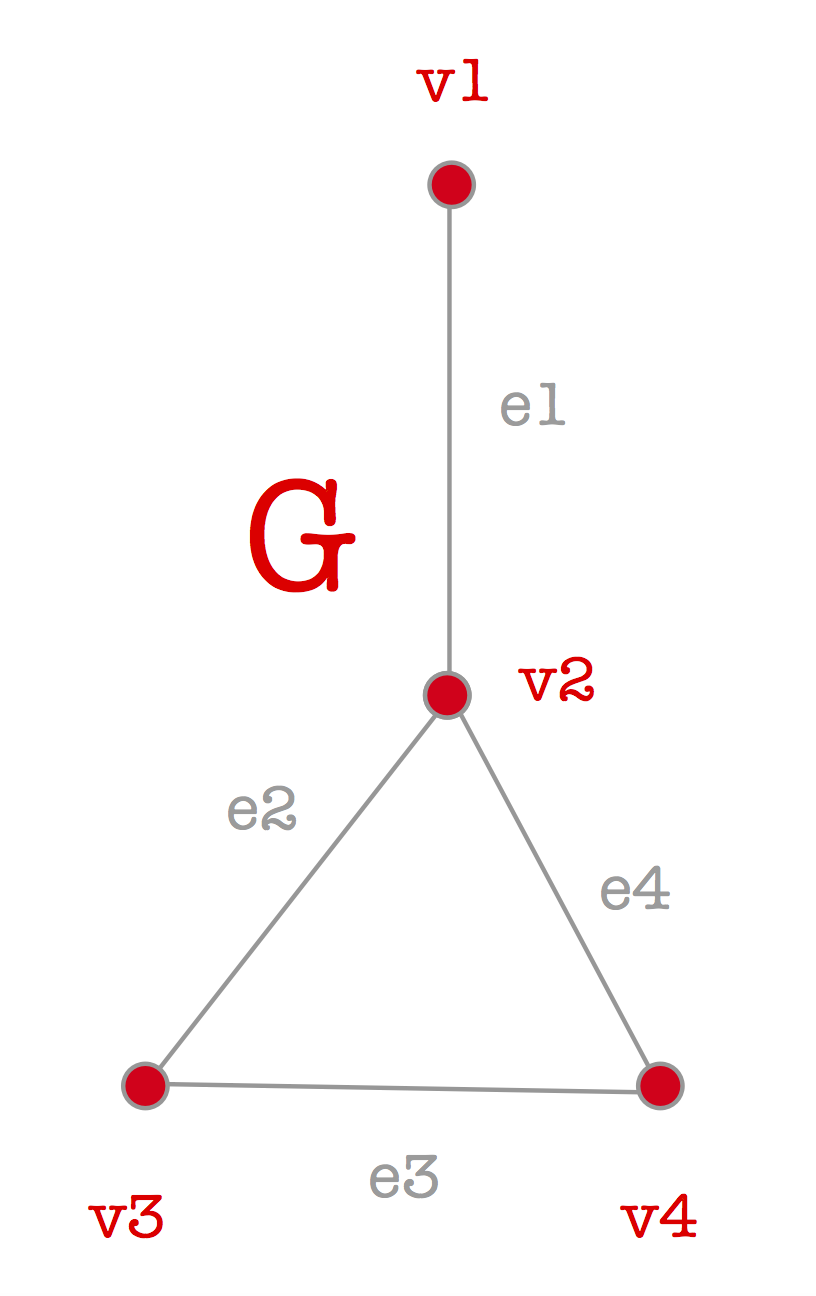
\includegraphics[height=3cm]{g3}
\end{figure}
\begin{itemize}
\item Aristas m\'ultiples: las aristas $e_4$ y $e_5$ se unen a los v\'ertices $v_3$ y $v_4$ (multigrafo).
\item Bucles: la arista $e_6$ une el v\'ertice $v_2$ con \'el mismo (pseudografo). 
\end{itemize}
\end{block}
\end{frame}




\begin{frame}
\frametitle{Definici\'on algebraica de grafo}

\begin{block}{Ejemplo}
N\'otese en este caso: 
\[E(G) = \{e_1=\{v_1,v_2\}, e_2=\{v_2,v_3\}, e_3 = \{v_1,v_4\}, \]
\[e_4 = \{v_3,v_4\}, e_5 = \{v_3,v_4\}, e_6 = \{v_2,v_3\}\}\]

$E(G)$ no es un conjunto, ya que tiene elementos repetidos $\{v_3,v_4\}$; es decir, las aristas $e_4$ y $e_5$ y la arista $e_6$ comienzan y acaban en el mismo v\'ertice. 

\end{block}
\end{frame}



\begin{frame}
\frametitle{Definici\'on algebraica de grafo}
La definici\'on de grafo dada anteriormente se corresponde con la definici\'on que diversos autores dan de \textbf{grafo simple}.  Y cuando se permiten aristas m\'ultiples y/o bucles como los del ejemplo anterior, se clasifica como \textbf{grafo general}. 
\end{frame}



\begin{frame}
\frametitle{Grafos dirigidos}
Otro concepto que resulta \'util es el de digrafo o grafo dirigido.
\begin{block}{Digrafo}
Sea $G$ un grafo simple (o grafo general). Si a cada arista se le asigna un sentido, se dir\'a que es un \textbf{digrafo}. 

\end{block}

\begin{figure}[h]
 \label{fig:volumen}
\centering
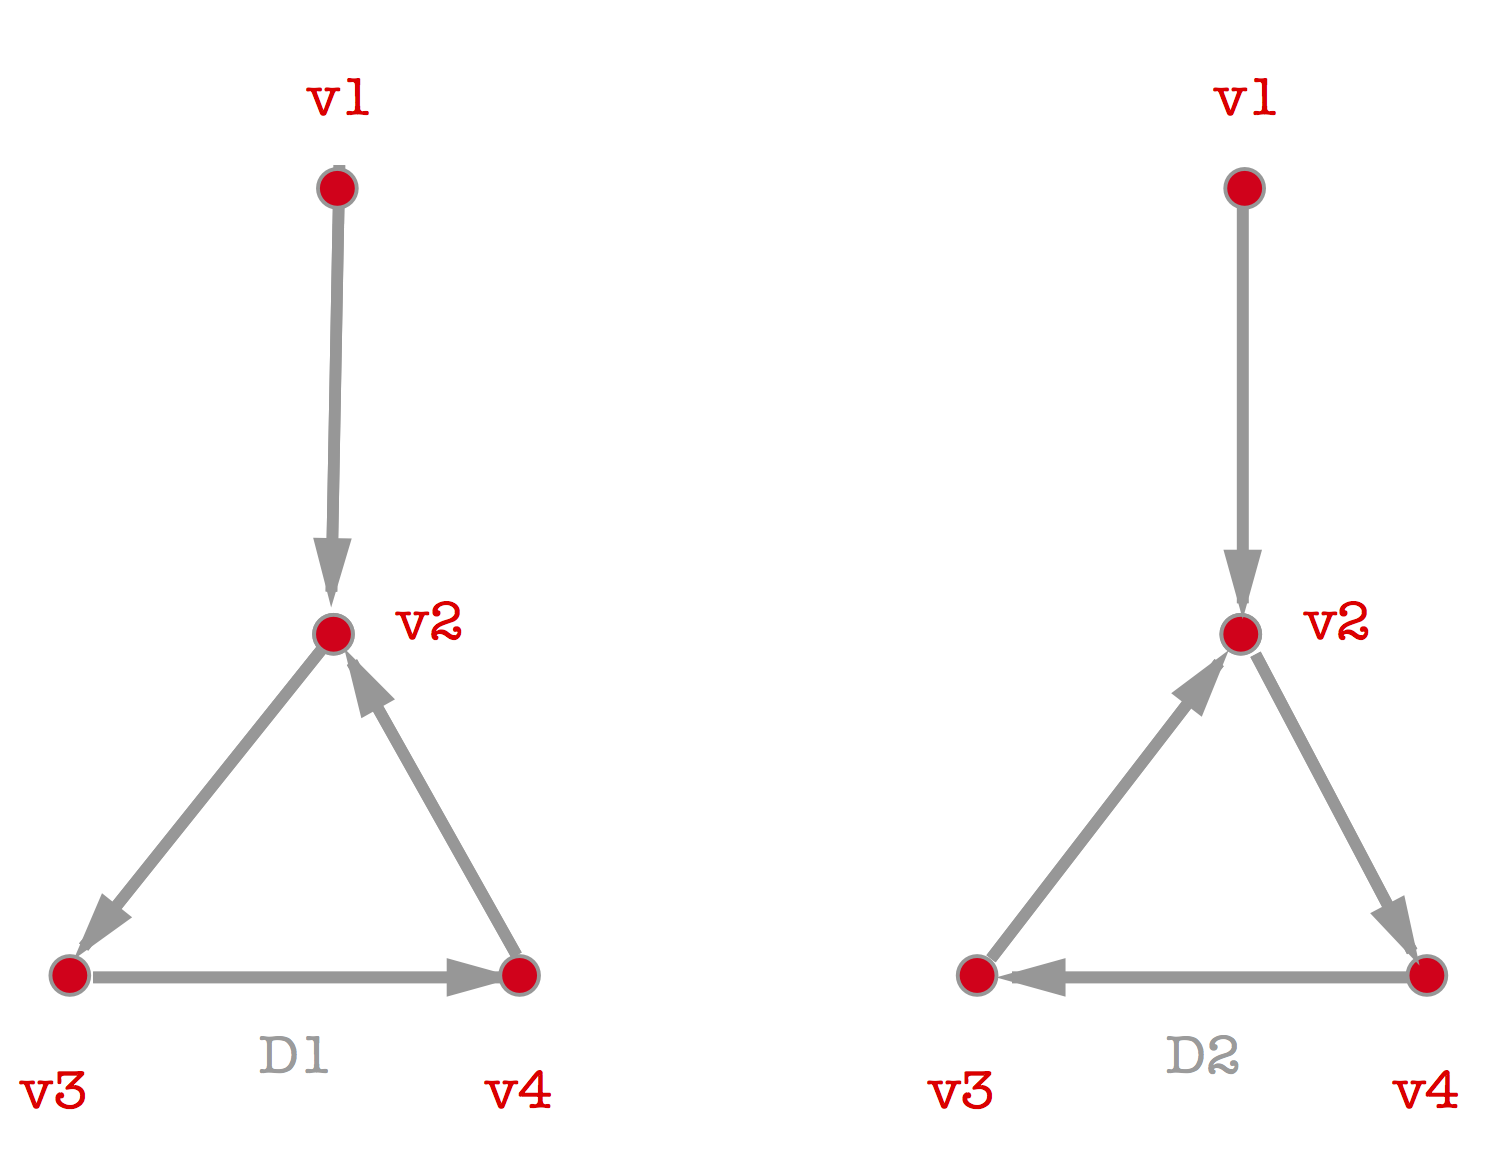
\includegraphics[height=4cm]{g5}
\end{figure}

Las aristas en estos casos son pares ordenados $D_1\neq D_2$.

\end{frame}





\begin{frame}
\frametitle{Grado de un v\'ertice}

\begin{block}{Ariastas incidentes}
D\'icese que una arista $e$ es \textbf{incidente} con un v\'ertice $v$ si $v$ es extremo de $e$.
\end{block}

\begin{block}{Grado de un v\'ertice}

El grado de un v\'ertice $v$, $gr(v)$ es igual al n\'umero de aristas que son incidentes con $v$.
\end{block}
\end{frame}




\begin{frame}
\frametitle{Grado de un v\'ertice}

Como cada arista es incidente a ambos v\'ertices, se tiene el siguiente resultado \'util:
\begin{block}{Teorema}
Sea $G=(V,E)$ un grafo, $V=\{v_1,v_2,\cdots, v_n\}$, entonces la suma de los grados de los v\'ertices de $G$ es igual al doble del n\'umero de aristas:
\[\displaystyle\sum_{i=1}^n gr(v_i) = 2|E|\]
\end{block}
\end{frame}



\begin{frame}
\frametitle{Grado de un v\'ertice}

\begin{block}{Ejemplo}
\begin{figure}[h]
 \label{fig:volumen}
\centering
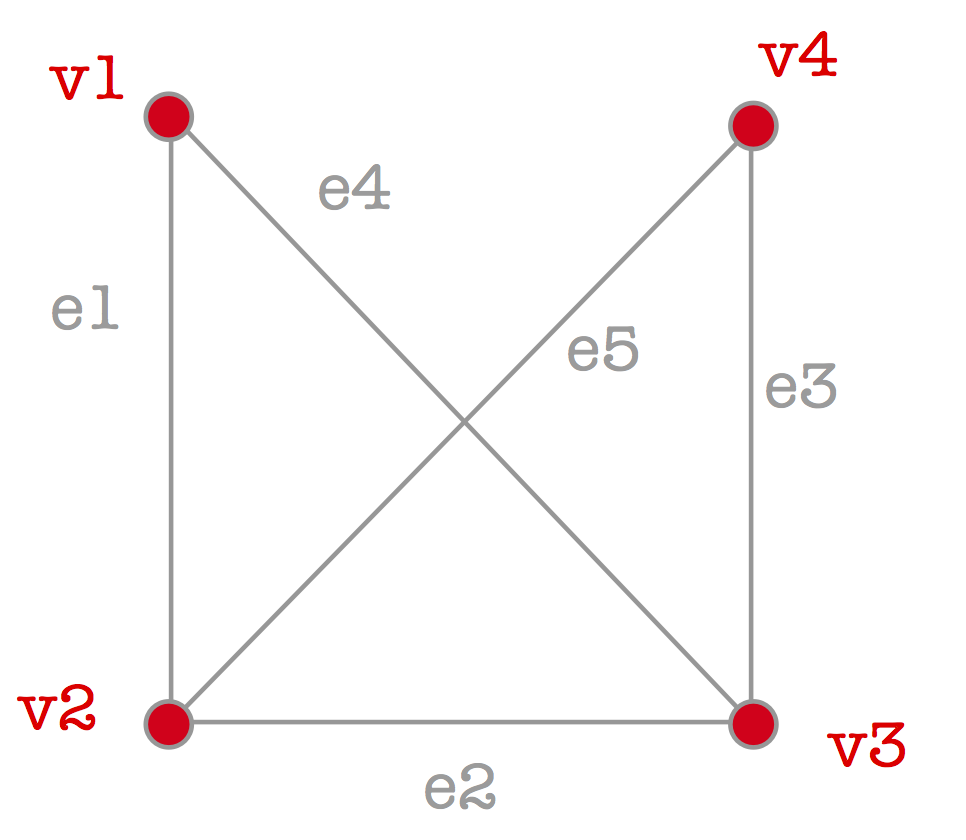
\includegraphics[height=3.5cm]{g6}
\end{figure}
\[gr(v_1) = 2\ \ gr(v_2) = 3\ \ gr(v_3) = 3\ \ gr(v_4) = 2\]
\[\displaystyle\sum_{i=1}^n gr(v_i) = 2 + 3 + 3 +2 = 10 = 2\cdot 5 =  2|E|\]
\end{block}
\end{frame}




\begin{frame}
\frametitle{Grado de un v\'ertice}

\begin{block}{Teorema}
Un v\'ertice es par o impar seg\'un su grado sea par o impar.
\end{block}

\begin{block}{Nota}
El teorema anterior tamb\'en es v\'alido para grafos generales.
\end{block}
\end{frame}




\begin{frame}
\frametitle{Grado de un v\'ertice}

\begin{block}{Ejemplo}
\begin{figure}[h]
 \label{fig:volumen}
\centering
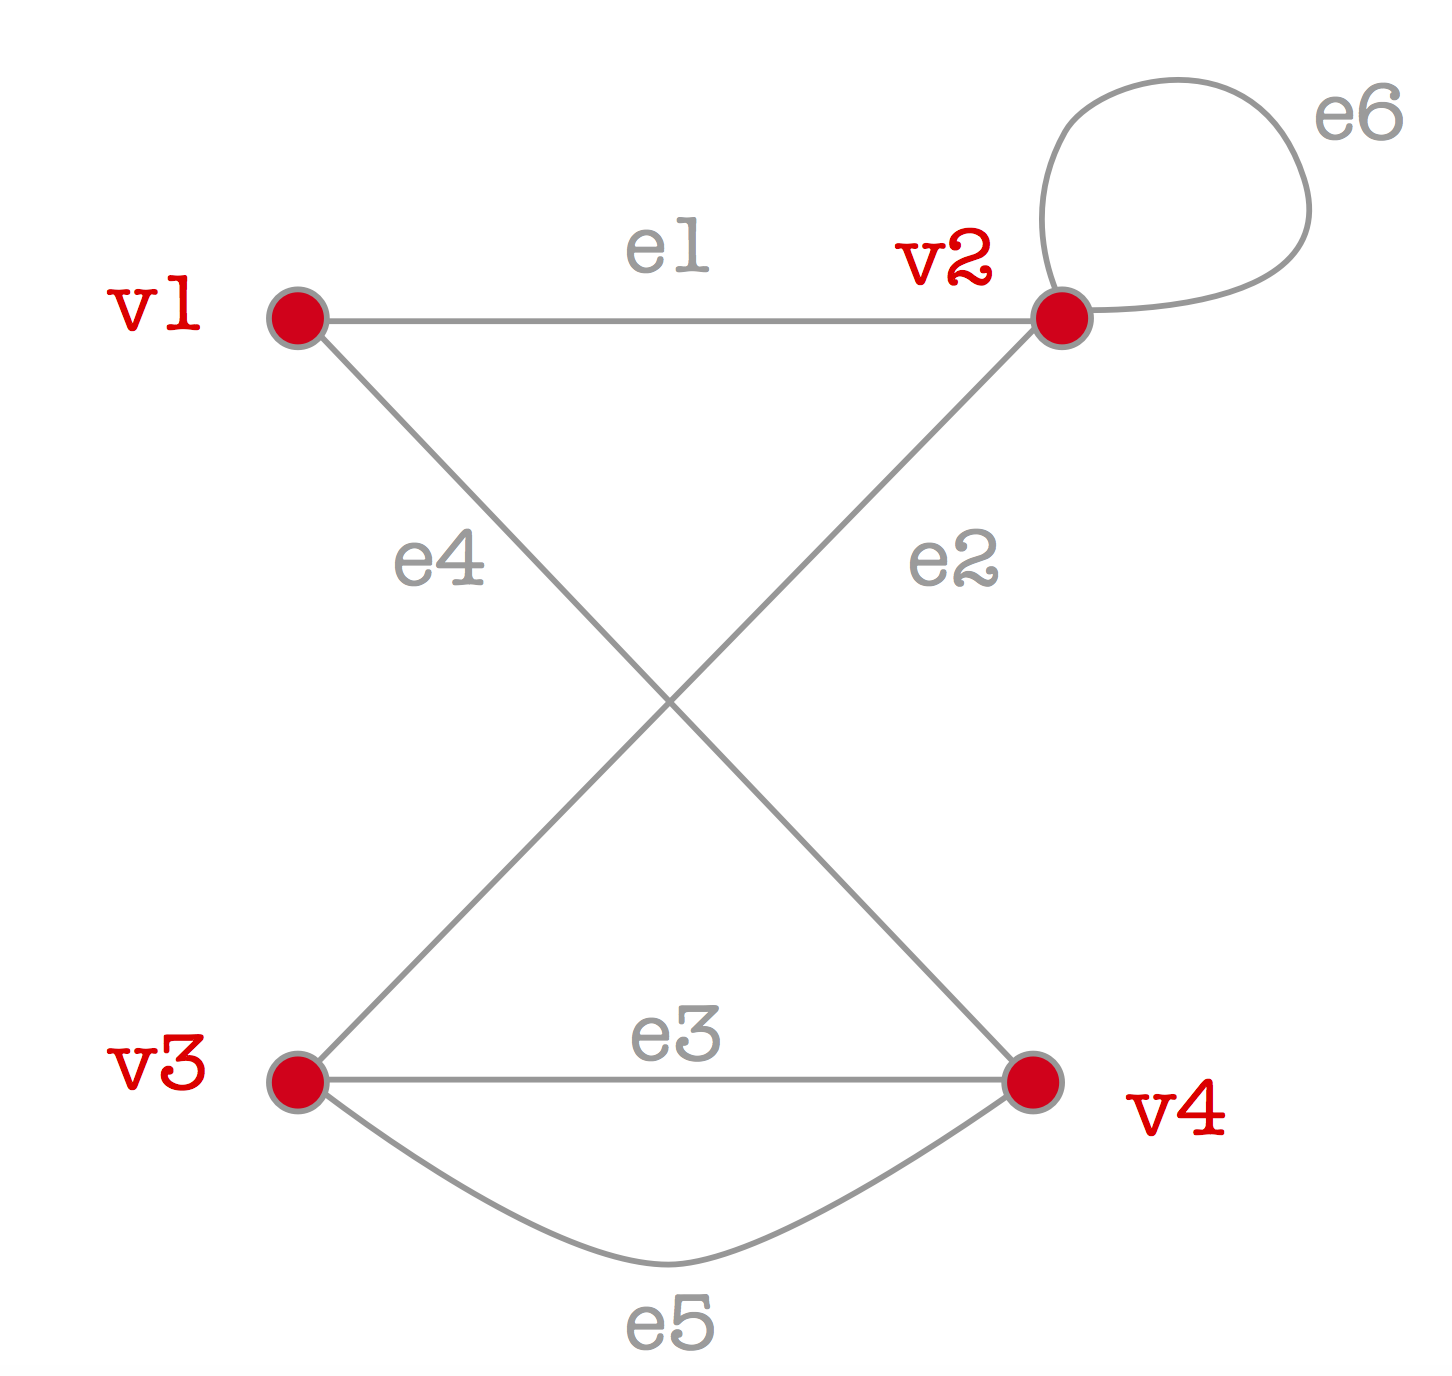
\includegraphics[height=3.5cm]{g4}
\end{figure}
\[gr(v_1) = 2\ \ gr(v_2) = 4\ \ gr(v_3) = 3\ \ gr(v_4) = 4\]
\[\displaystyle\sum_{i=1}^n gr(v_i) = 2 + 4 + 3 +3 = 12 = 2\cdot 6 =  2|E|\]
\end{block}
\end{frame}



\begin{frame}
\frametitle{Grado de un v\'ertice}

\begin{block}{Ejercicios}
\begin{enumerate}
\item Dib\'ujese, si es posible, un grafo con 5 v\'ertices, de manera que el grado de cada v\'ertice sea 3. 
\item Dib\'ujese, si es posible, un grafo con 5 v\'ertices, de manera que el grado de cada v\'ertice sea 2. 
\end{enumerate}
\end{block}
\end{frame}




\begin{frame}
\frametitle{Caminoss}
En un grafo que represente, por ejemplo, una red de comunicaciones es importante conocer la existencia de caminos que recorren todas las aristas o todos los v\'ertices y que, en cierta manera, sean los m\'as econ\'omicos. Para eso se van a ver las siguientes definiciones b\'asicas (la nomenclatura que se da aqu\'i no es \'unica, hay autores que dan nombres diferentes):
\end{frame}


\begin{frame}
\frametitle{Caminos}
\begin{block}{Definici\'on}
Un camino en un grafo $G$ es una secuencia finita alternada de v\'ertices y aristas de $G$:
\[v_0\rightarrow e_1 = \{v_0,v_1\}\rightarrow v_1 \rightarrow e_2 = \{v_1,v_2\} \cdots  e_n = \{v_{n-1},v_n\}\rightarrow v_n\]
\[v_0,e_1,v_1,e_2\cdots e_n,v_n\]
Donde cada arista tiene por extremo los v\'ertices inmediatamente precedentes o siguientes de la secuencia. Por lo que el camino tambi\'en se puede representar por la secuencia de v\'ertices $v_0,v_1,\cdots,v_n$.
\end{block}
\end{frame}



\begin{frame}
\frametitle{Caminos}
\begin{block}{Extremos del camino}
Los v\'ertices $v_0$ y $v_n$ se denomina extremos del camino y se dice que el camino va de $v_0$ a $v_n$ o que conecta $v_0$ con $v_n$.
\end{block}

\begin{block}{Longitud del camino}

La longitud del camino es el n\'umero de aristas que contiene.
\end{block}
\end{frame}





\begin{frame}
\frametitle{Caminos}
\begin{block}{Clasificaci\'on de los caminos}
\begin{itemize}
\item Recorrido: camino sin aristas repetidas.
\item Camino simple: recorrido sin v\'ertices repetidos excepto el primero y el \'ultimo.
\item Camino cerrado: camino en el cual sus dos extremos coinciden. Es decir, comienza y acaba en el mismo v\'ertice. en caso contrario el camino es abierto.
\item Circuito: recorrido cerrado.
\item Ciclo: circuito que tambi\'en es camino simple.
\end{itemize}
\end{block}
\end{frame}






\begin{frame}
\frametitle{Caminos}
\begin{block}{Clasificaci\'on de los caminos}
Dado el grafo, clasif\'iquense los siguientes caminos:
\begin{figure}[h]
 \label{fig:volumen}
\centering
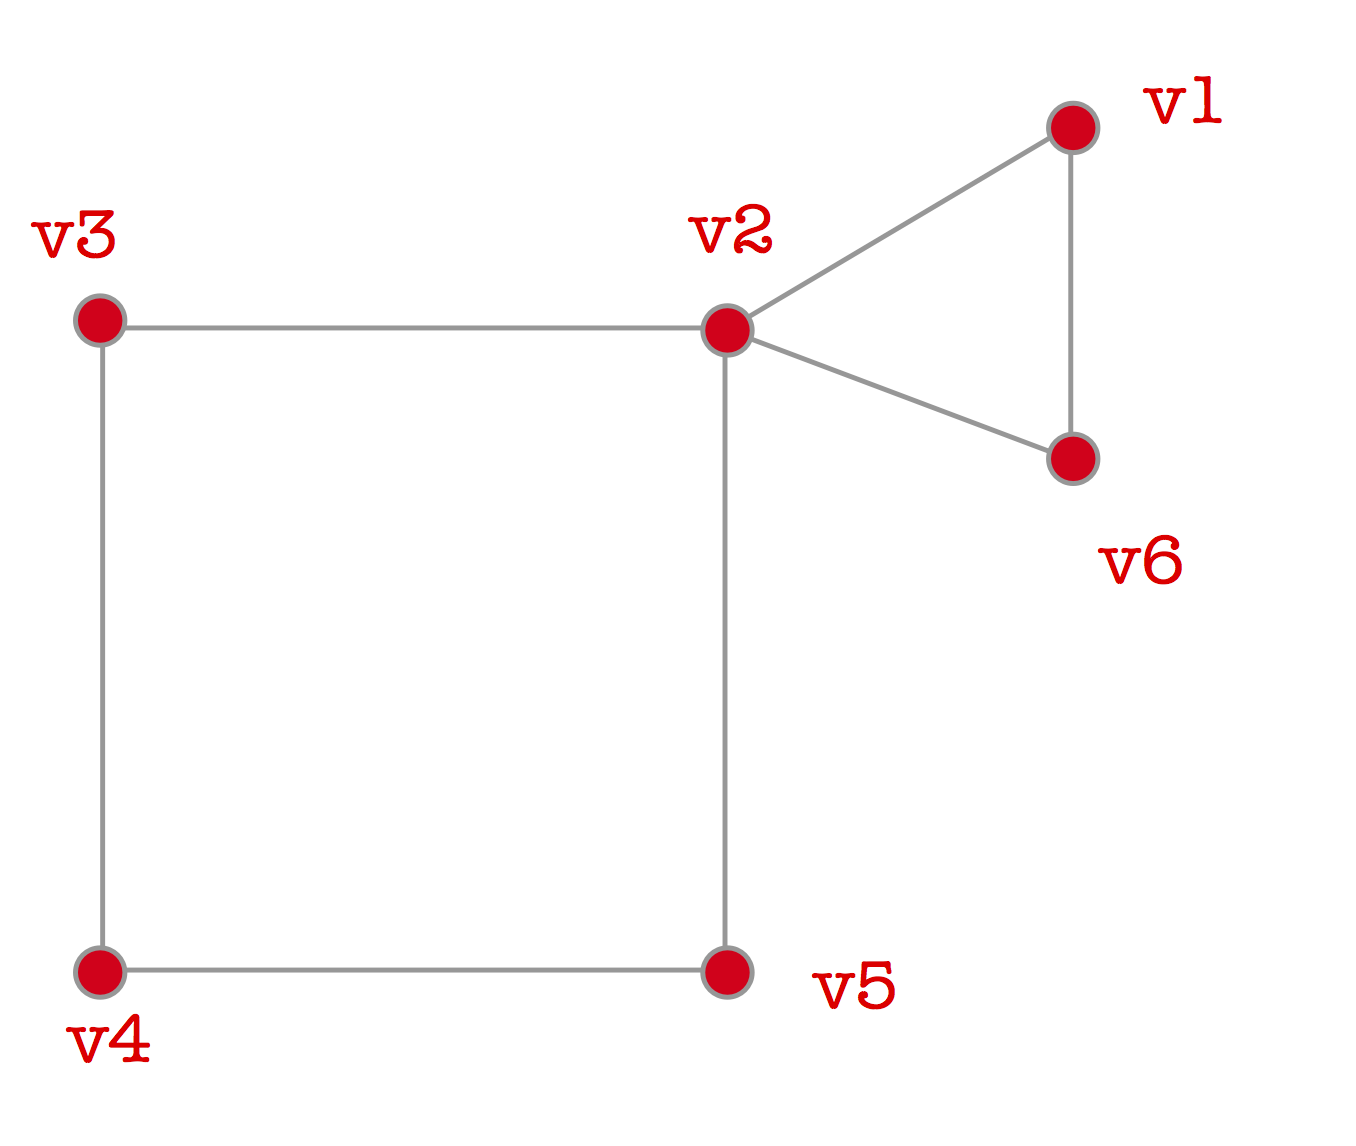
\includegraphics[height=3cm]{g7}
\end{figure}
\end{block}
\end{frame}



\begin{frame}
\frametitle{Caminos}
\begin{block}{Clasificaci\'on de los caminos}
\begin{itemize}
\item $v_2v_3v_4v_5v_2$
\item $v_2v_3v_4v_5$
\item $v_6v_2v_3v_4v_5v_2v_1v_6$
\item $v_1v_2v_6v_1$
\end{itemize}
\end{block}
\end{frame}





\begin{frame}
\frametitle{Conectividad}
Existen grafos en los cuales para cada par de v\'ertices $v_i,v_j$ hay, al menos, un posible camino que los conecta y otros casos en los cuales es imposible unir dos v\'ertices dados.
\end{frame}


\begin{frame}
\frametitle{Conectividad}
\begin{block}{Grafo conexo}
Un grafo $G$ d\'icese conexo si existe un camino simple entre cualquier par de v\'ertices $v_i,v_j$.

En caso contrario, el grafo es no conexo y los v\'ertices $v_i$ y $v_j$ pertenecen a diferentes componentes conexas del grafo.
El n\'umero de componentes conexos de un grafo se denota por $K(G)$.
\end{block}
\end{frame}





\begin{frame}
\frametitle{Conectividad}
\begin{block}{Ejemplo}

\begin{figure}[h]
 \label{fig:volumen}
\centering
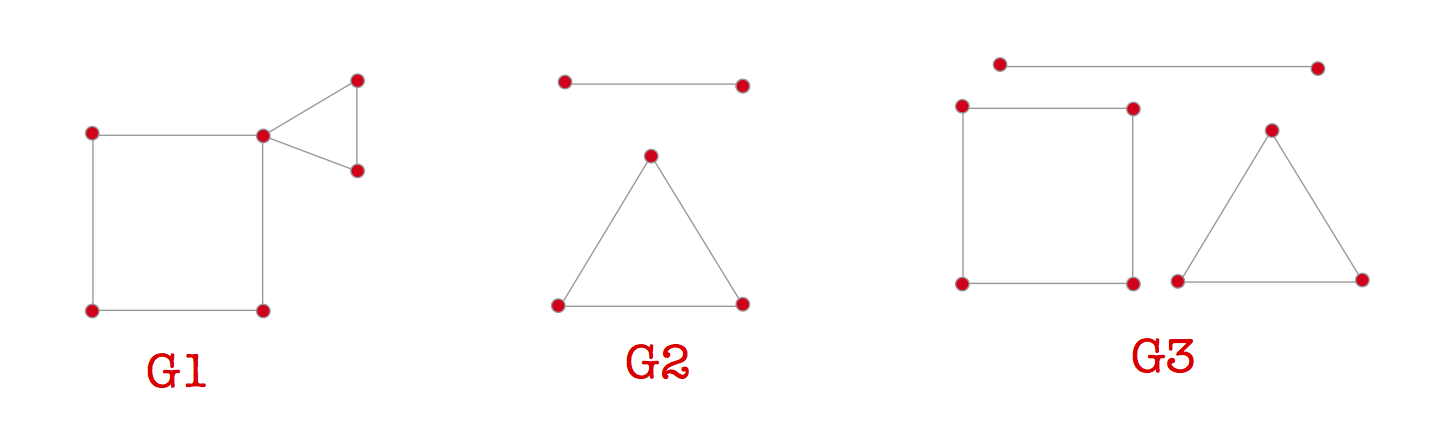
\includegraphics[height=3cm]{g8}
\end{figure}

$G_1$ es un grafo conexo, mientras que $G_2$ y $G_3$ no lo son. $K(G_1) = 1, K(G_2) = 2, K(G_3) = 3$.
\end{block}
\end{frame}





\section{Grafos y matrices}
\subsection{Representaci\'on matricial}

\begin{frame}
\frametitle{Representaci\'on matricial de los grafos}
\begin{block}{Definici\'on}
Sea $G=(V,E)$ un grafo simple con $V=\{v_1,v_2,\cdots,v_n\}$. Se define su matriz de adyacencia como la matriz cuadrada:
\[A(G) = (a_{ij})_{n\times n} = \left\{\begin{array}{ll}1 & si\ v_i\ y\ v_j\ son\ adyacentes \\0 & en\ otro\ caso\end{array}\right.\]

\end{block}
N\'otese que $A(G)$ es una matriz sim\'etrica y que $a_{ii} = 0\ \forall\ i=1,\cdots,n$.

La matriz de adyacencia no es \'unica (depende de la ordenaci\'on de los v\'ertices). 
\end{frame}


\begin{frame}
\frametitle{Representaci\'on matricial de los grafos}
\begin{block}{Definici\'on}
\begin{itemize}
\item Si $G=(V,E)$ es un grafo general $V=\{v_1,v_2,\cdots,v_n\}$, se define $A(G) = (a_{ij})_{n\times n}$ donde $a_{ij}$ es el n\'umero de aristas que unen $v_i$ con $v_j$. Entonces, $A(G)$ es sim\'etrica.
\item Si $G=(V,E)$ es un digrafo $V=\{v_1,v_2,\cdots,v_n\}$, se define $A(G) = (a_{ij})_{n\times n}$ donde $a_{ij}$ es el n\'umero de aristas que unen $v_i$ con $v_j$. Entonces, $A(G)$ no es sim\'etrica.

\end{itemize}
\end{block}
\end{frame}



\begin{frame}
\frametitle{Representaci\'on matricial de los grafos}
\begin{block}{Ejemplo}
\begin{figure}[h]
 \label{fig:volumen}
\centering
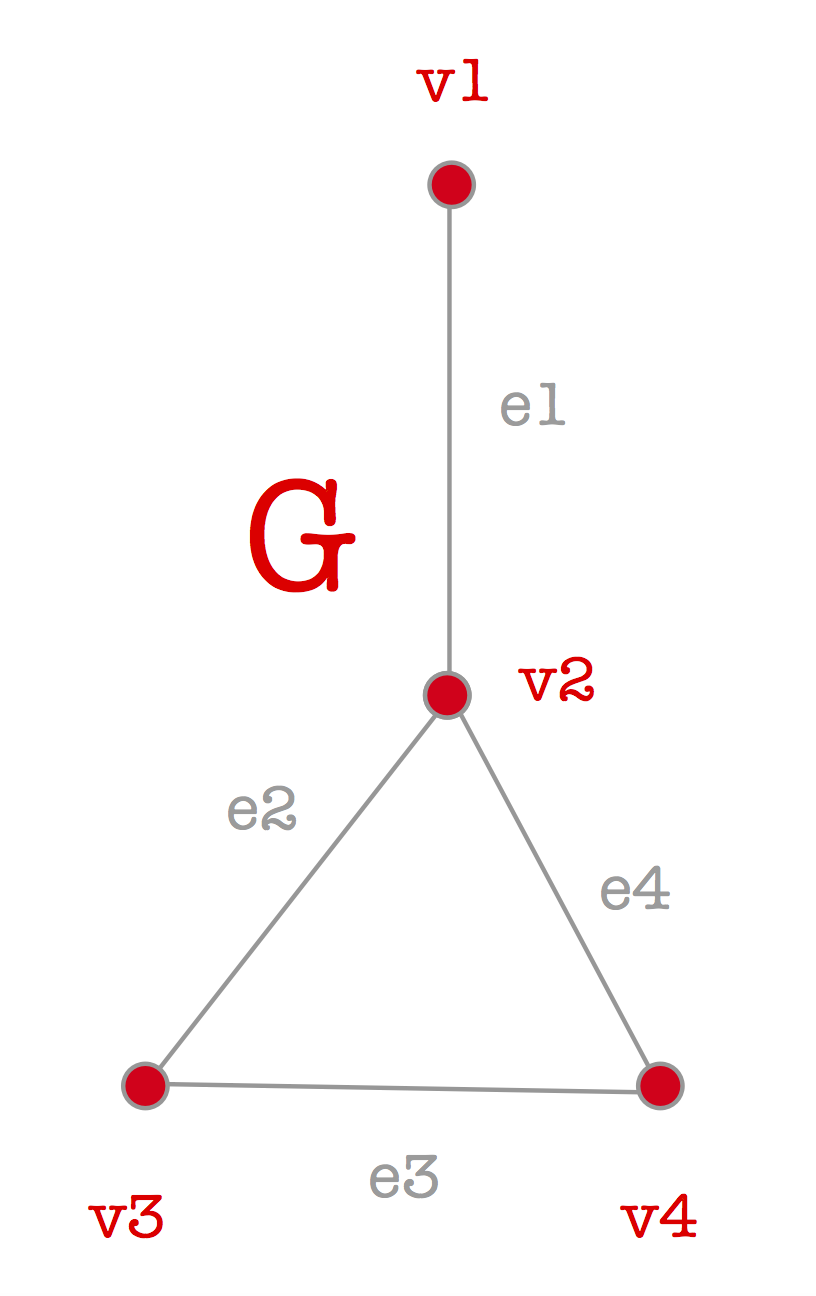
\includegraphics[height=3cm]{g3}
\end{figure}

\[A(G) = \left(\begin{array}{cccc}a_{11} & a_{12} & a_{13} & a_{14} \\a_{21} & a_{22} & a_{23} & a_{24} \\a_{31} & a_{32} & a_{33} & a_{34} \\a_{41} & a_{42} & a_{43} & a_{44}\end{array}\right) = \left(\begin{array}{cccc}0 & 1 & 0 & 0 \\1 & 0 & 1 & 1 \\0 & 1 & 0 & 1 \\0 & 1 & 1 & 0\end{array}\right)\]
Con $a_{ij}\in\{0,1\}$ y $a_{ii} = 0$
\end{block}
\end{frame}



\begin{frame}
\frametitle{Representaci\'on matricial de los grafos}
\begin{block}{Ejemplo}
\begin{figure}[h]
 \label{fig:volum}
\centering
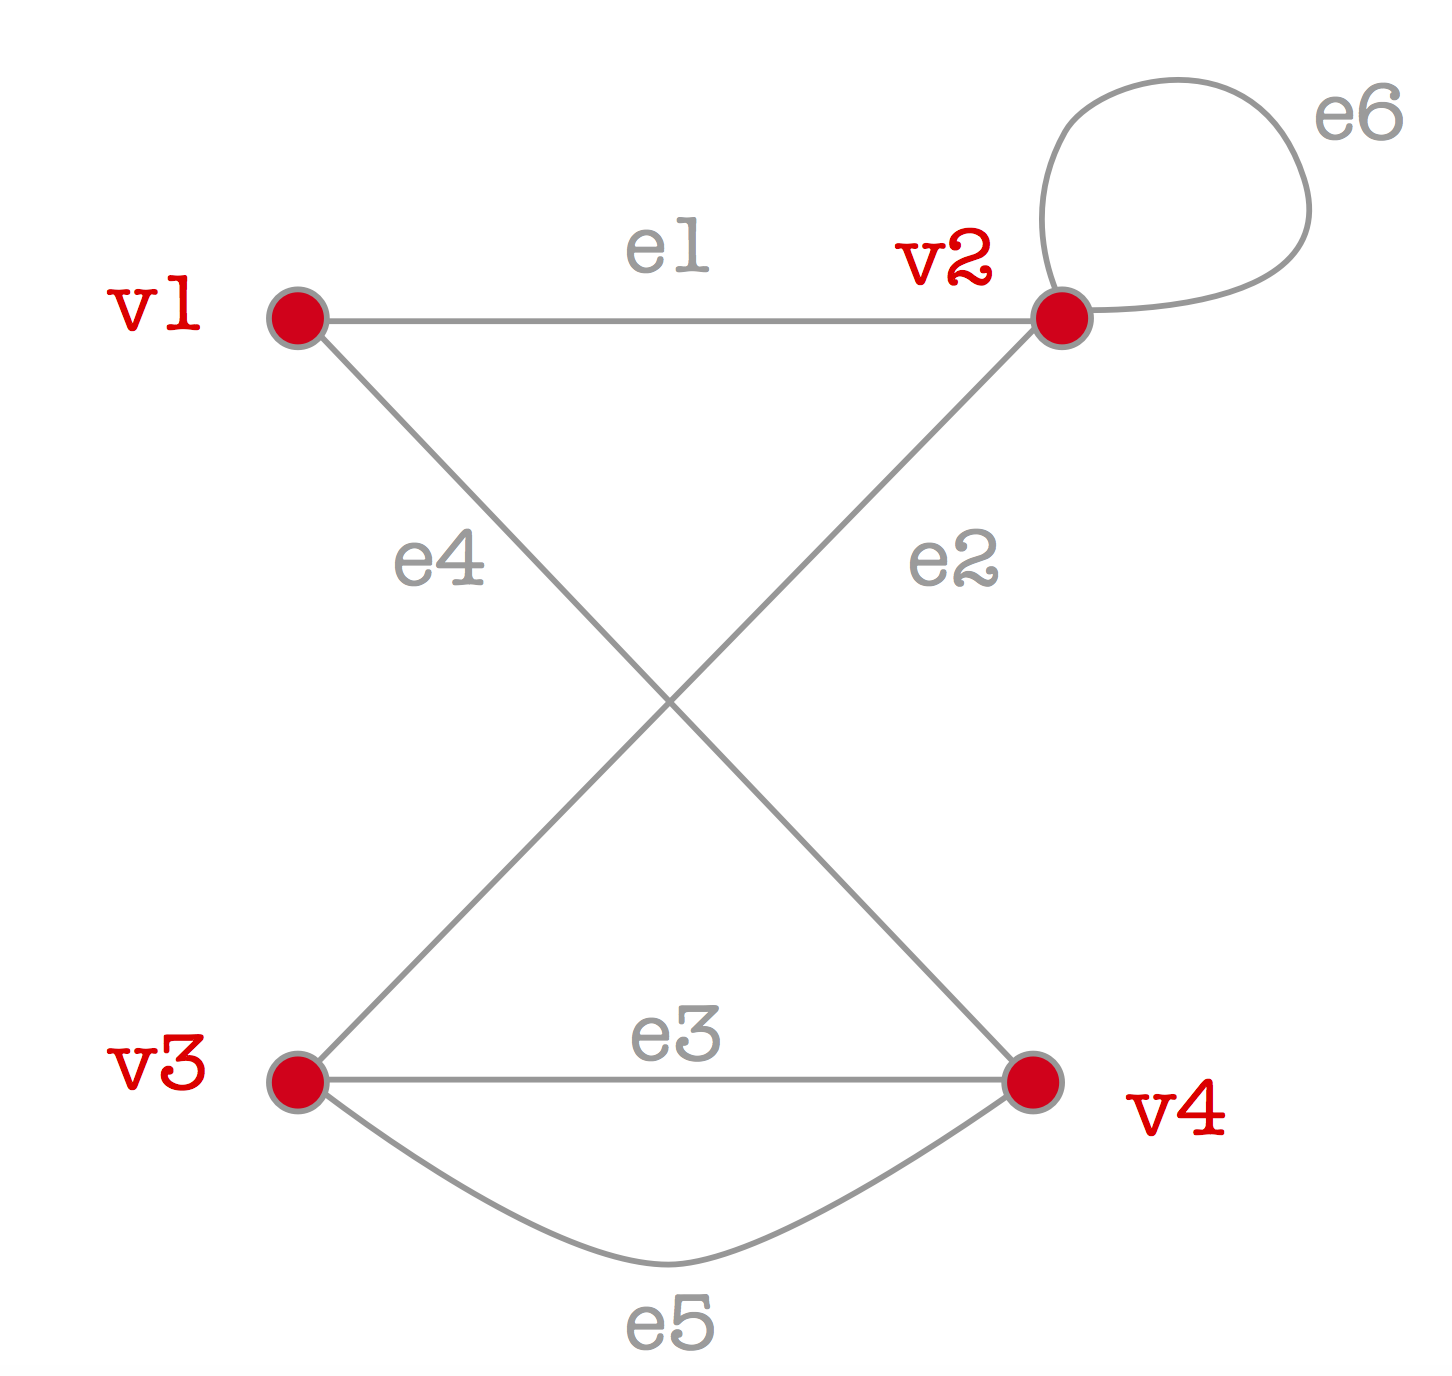
\includegraphics[height=2.5cm]{g4}
\end{figure}
\[A(G) = \left(\begin{array}{cccc}a_{11} & a_{12} & a_{13} & a_{14} \\a_{21} & a_{22} & a_{23} & a_{24} \\a_{31} & a_{32} & a_{33} & a_{34} \\a_{41} & a_{42} & a_{43} & a_{44}\end{array}\right) = \left(\begin{array}{cccc}0 & 1 & 0 & 1 \\1 & 1 & 1 & 0 \\0 & 1 & 0 & 2 \\1 & 0 & 2 & 0\end{array}\right)\]
En este caso $a_{ij}$ puede ser m\'as grande que $1$ ya que el grafo tiene aristas m\'ultiples y $a_{ii}\neq 0$ (bucles)
\end{block}
\end{frame}






\begin{frame}
\frametitle{Representaci\'on matricial de los grafos}
\begin{block}{Teorema}
Sea $A(G)$ la matriz de adyacencia de un grafo con $n$ v\'ertices. Entonces la entrada $(i,j)$ de la matriz $A^m$ nos dar\'a el n\'umero de caminos de longitud $m$ que conecten los v\'ertices $v_i$ y $v_j$.  
\end{block}
\end{frame}




\begin{frame}
\frametitle{Representaci\'on matricial de los grafos}
\begin{block}{Ejemplo}
Si se considera la matriz del ejemplo anterior:
\[A(G) = \left(\begin{array}{cccc}a_{11} & a_{12} & a_{13} & a_{14} \\a_{21} & a_{22} & a_{23} & a_{24} \\a_{31} & a_{32} & a_{33} & a_{34} \\a_{41} & a_{42} & a_{43} & a_{44}\end{array}\right) = \left(\begin{array}{cccc}0 & 1 & 0 & 0 \\1 & 0 & 1 & 1 \\0 & 1 & 0 & 1 \\0 & 1 & 1 & 0\end{array}\right)\]
Se tiene que:
\[A^2(G) = \left(\begin{array}{cccc}1 & 0 & 1 & 1 \\0 & 3 & 1 & 1 \\1 & 1 & 2 & 1 \\1 & 1 & 1 & 2\end{array}\right); \ A^3(G) = \left(\begin{array}{cccc}0 & 3 & 1 & 4 \\3 & 2 & 4 & 4 \\1 & 4 & 2 & 3 \\1 & 4 & 3 & 2\end{array}\right)\]

\end{block}
\end{frame}


\begin{frame}
\frametitle{Representaci\'on matricial de los grafos}
\begin{block}{Ejemplo}
Consid\'erese por ejemplo el elemento $a_{14}$ de estas tres matrices. 
\begin{itemize}
\item El elemento $a_{14}$ de $A(G)$ es cero, eso indica que no hay ning\'un camino entre los v\'ertices $v_1$ y $v_4$, pero eso no indica que no se puedan conectar estos v\'ertices.

\item El elemento $a_{14} \in A^2(G)$ toma el valor $1$, indicando as\'i que existe un camino de longitud $2$ que conecta $v_1$ y $v_4$. Este camino ser\'a:
 $v_1v_2v_4$.

\item El elemento $a_{14}\in A^3(G)$ toma el valor $1$, entonces existe un camino de longitud $3$ que conecta $v_1$ y $v_4$. Este camino ser\'a $v_1v_2v_3v_4$.
\end{itemize}
\end{block}
\end{frame}

\subsection{Isomorfismo de grafos}

\begin{frame}
\frametitle{Isomorfismo de grafos}
\begin{block}{Definici\'on}
Sean $G(V,E)$ y $G'(V',E')$ dos grafos (o grafos generales sin bucles) y $f:V\longrightarrow V'$ una aplicaci\'on biyectiva tal que \[\{u,v\}\in E \Longleftrightarrow \{f(u),f(v)\}\in E'\]
Entonces se dir\'a que $f$ es un isomorfismo entre $G$ y $G'$ o que $G$ y $G'$ son grafos isomorfos. 
\end{block}
En general no es f\'acil determinar cuando dos grafos son o no son isomorfos.

Es claro que si dos grafos son isomorfos han de tener el mismo n\'umero de v\'ertices e igual n\'umero de aristas, pero eso no es suficiente. 
\end{frame}

\begin{frame}
\frametitle{Isomorfismo de grafos}
\begin{block}{Teorema}
Si $G$ y $G'$ son grafos isomorfos, entonces:
\[si\ v\in V \Longrightarrow gr(v) = gr(f(v))\]
\end{block}
\end{frame}



\begin{frame}
\frametitle{Isomorfismo de grafos}
\begin{block}{Ejemplo}
\begin{figure}[h]
 \label{fig:volumen}
\centering
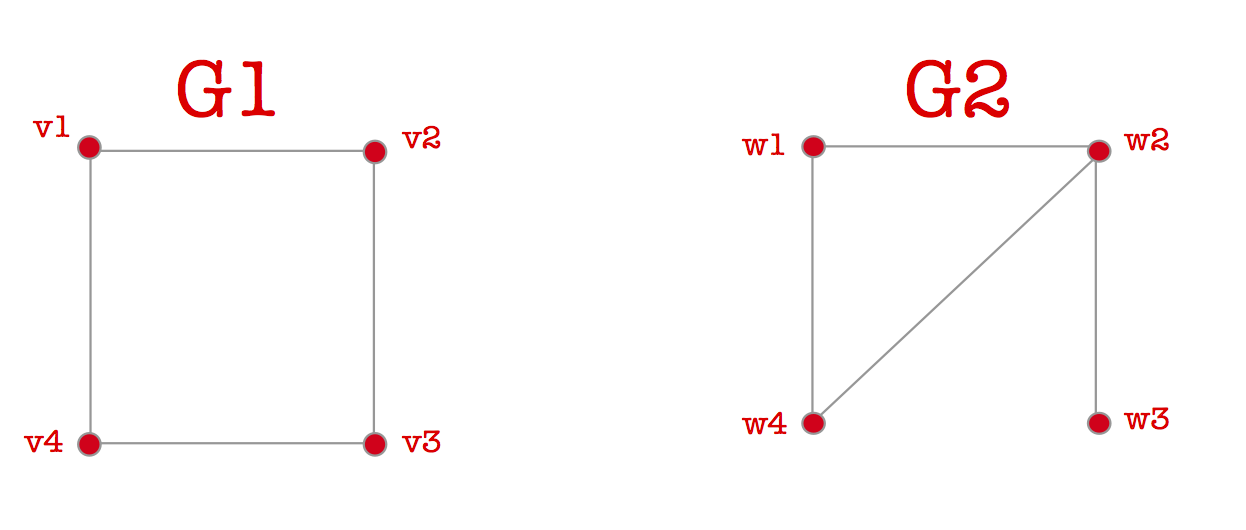
\includegraphics[height=3cm]{g9}
\end{figure}
$G$ y $G'$ tienen el mismo n\'umero de v\'ertices y el mismo n\'umero de aristas.

$\forall \ v\in V(G),\ gr(v) = 2$, pero en cambio $gr(w_3) = 1$, por tanto $G$ y $G'$ no pueden ser isomorfos. 
\end{block}
\end{frame}





\subsection{Grafos de Euler y grafos de Hamilton}

\begin{frame}
\frametitle{Grafos de Euler}
\begin{block}{Definici\'on}
Sea $G$ un grafo conexo
\begin{itemize}
\item Un camino euleriano es un recorrido en el cual aparecen todas las aristas. 
\item Un circuito euleriano es un camino euleriano cerrado.
\item Un grafo euleriano es un grafo con un circuito euleriano.
\end{itemize}
\end{block}
\end{frame}


\begin{frame}
\frametitle{Grafos de Euler}
\begin{block}{Teorema}
Sea $G$ un grafo entonces:
\begin{itemize}
\item Si $G$ tiene un circuito euleriano, el grado de cada v\'ertice es par.
\item Si $G$ tiene un camino euleriano, el grafo $G$ tiene exactamente dos v\'ertices de grado impar (exactamente los v\'ertices donde comienza y acaba el camino).
\end{itemize}
\end{block}
\end{frame}




\begin{frame}
\frametitle{Grafos de Euler}
\begin{block}{Ejemplos}
Consid\'erese el grafo siguiente:
\begin{figure}[h]
 \label{fig:volumen}
\centering
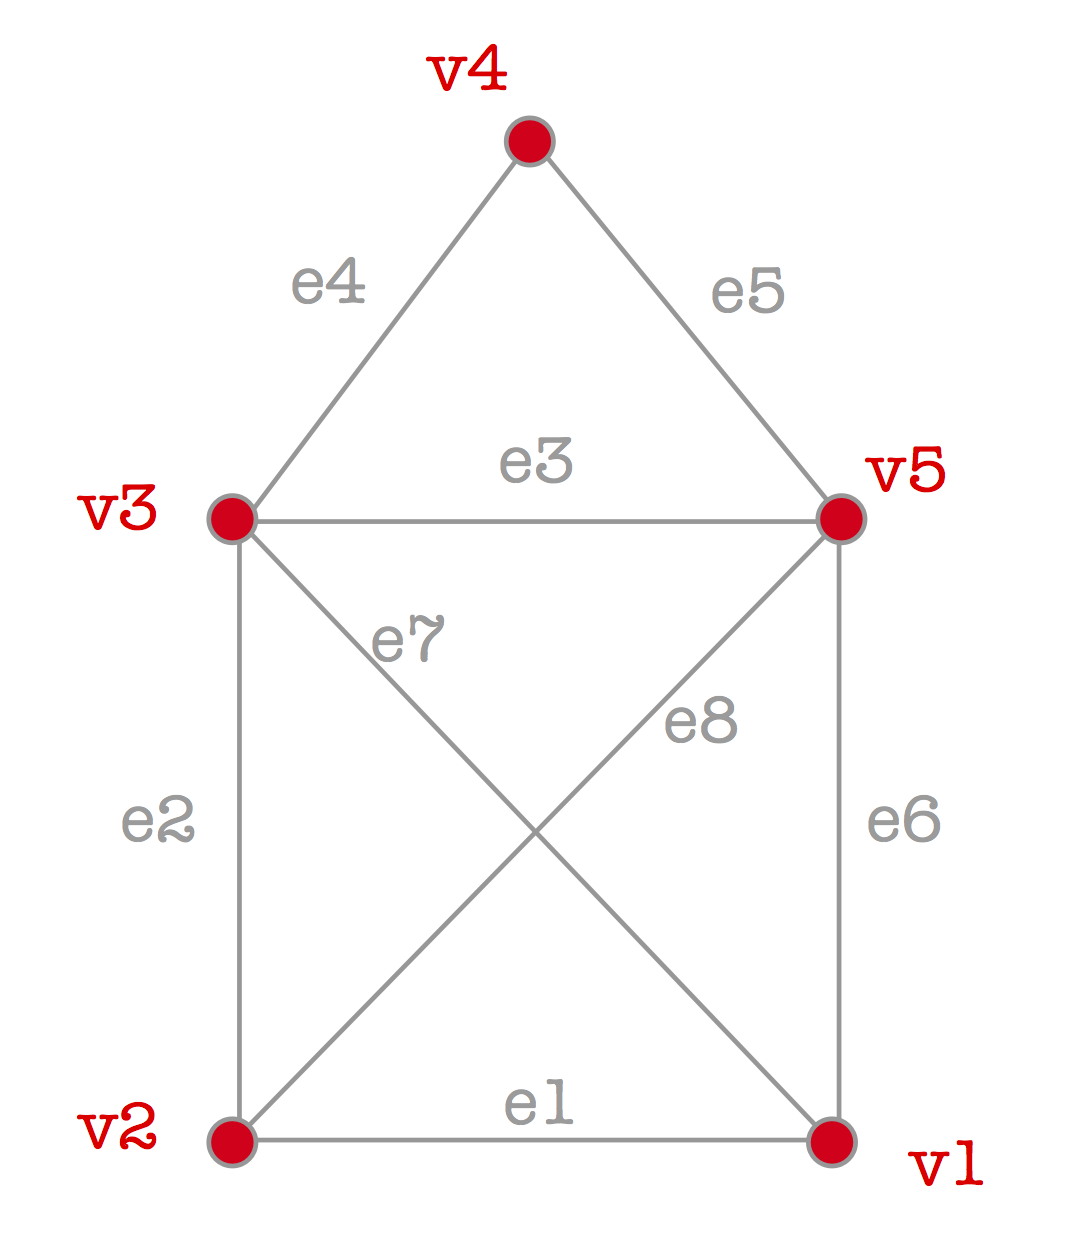
\includegraphics[height=2.5cm]{g10}
\end{figure}
La secuencia $e_2$ $e_4$ $e_5$ $e_8$ $e_1$ $e_7$ $e_3$ $e_6$ es un camino euleriano.

\[gr(v_1)=3,gr(v_2)=3,gr(v_3)=4,gr(v_4)=2,gr(v_5)=4\]

Teniendo dos v\'ertices de grado 3, el camino comienza en uno de ellos y acaba en el otro. 

\end{block}
\end{frame}







\begin{frame}
\frametitle{Grafos de Euler}
\begin{block}{Ejemplo}
Consid\'erese el grafo que representa los puentes de K\"onigsberg. 
\begin{figure}[h]
 \label{fig:volumen}
\centering
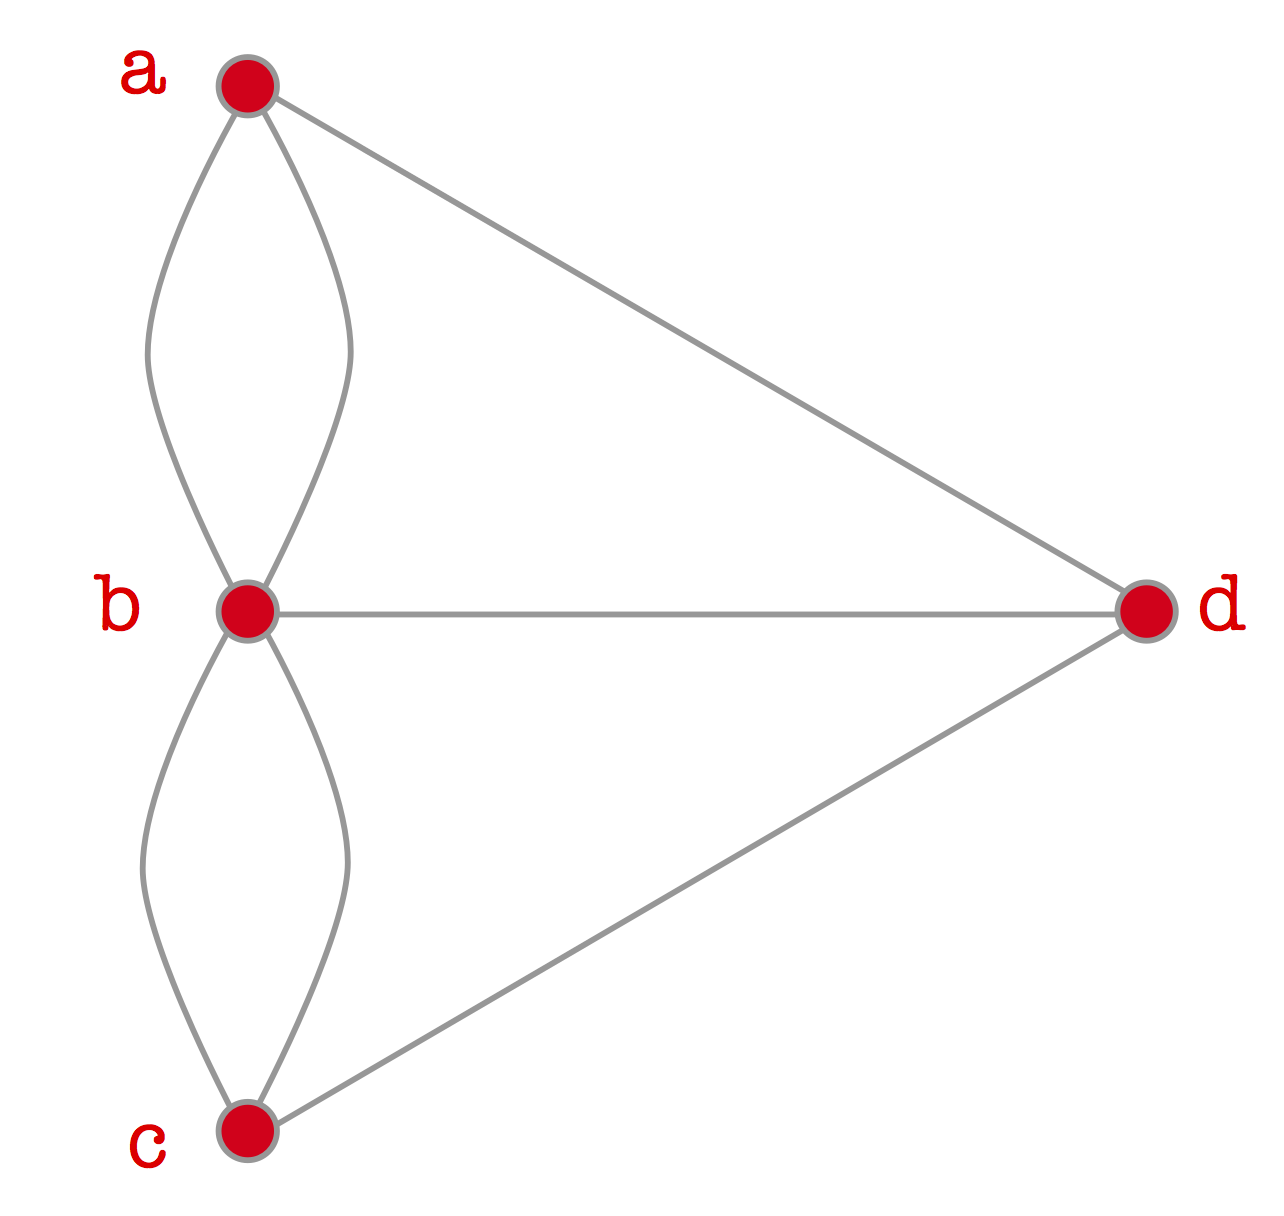
\includegraphics[height=3cm]{g11}
\end{figure}

Se observa que $a,c$ y $d$ tienen grado 3 y que $b$ tiene grado 5. Como todos los v\'ertices tienen grado impar se puede deducir que no existe ning\'un circuito euleriano. Por tanto el problema de los puentes de K\"onigsberg no tiene soluci\'on. 
\end{block}
\end{frame}





\begin{frame}
\frametitle{Grafos de Hamilton}
\begin{block}{Definici\'on}
Sea $G$ un grafo:

\begin{itemize}
\item Un camino de Hamilton es un camino que recorre todos los v\'ertices solo una vez. 
\item Un circuito de Hamilton es un camino de Hamilton cerrado (recorre todos los v\'ertices solo una vez salvo los extremos). 
\item Un grafo con un circuito de Hamilton se denomina un grafo de Hamilton. 
\end{itemize}
\end{block}
\end{frame}

%\begin{tabular}{ |p{1cm}||p{0.8cm}|p{0.8cm}|p{0.8cm}|p{0.8cm}|p{0.8cm}|p{0.8cm}|p{1.6cm}|  }
% \hline
% Z & $x_1$ & $x_2$ & $s_1$& $s_2$ & $v_1$  & $v_2$& Constantes \\
% \hline
%1 &0 & 130 & -100 & 33& 0& -133 & 404 \\
%0 & 0 &  4/3 & -1 & 1/3 & 1 & -1/3 & 4 \\
%0 & 1 & 2/3 & 0 & -1/3 & 0 & 1/3  & 4 \\
% \hline
%\end{tabular}
%\end{frame}


%  \begin{figure}[h]
  %  \label{fig:volumen}
%\centering
%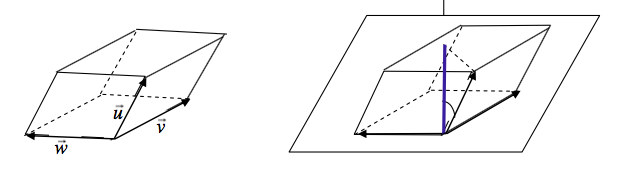
\includegraphics[height=3cm]{volum}
%\end{figure}


\end{document}